\section{Introduction}
\label{sec:intro}

% Climate and weather models are expensive, and we really want ensembles
Weather and climate prediction requires the integration of a computational
model derived from the fundamental equations of motion and initialized
with an estimate of the present-day system state (e.g., temperature, wind speeds,
etc.).
Due to the high computational cost of the physical model, prediction systems
typically require suboptimal tradeoffs.
On one hand, it is desirable to increase the credibility of the underlying
numerical model as much as possible,
for instance by increasing model grid resolution
\citep <e.g.,>[]{hewitt_impact_2016}
or by explicitly
simulating as many coupled components (e.g., atmosphere, land, ocean, ice) as
possible \citep <e.g.,>[]{penny_coupled_2017}.
On the other hand, knowledge of the model initial conditions is imperfect and
the governing equations will always contain necessary, inexact approximations of
reality.
As a result, prediction systems employ
statistical methods like ensemble based forecasting in order to represent this
uncertainty.
Producing an ensemble with statistical significance
requires integrating the underlying numerical model many times; usually
$\mathcal{O}(10-100)$ in practice, but ideally $>1,000$
\citep{evensen_data_2022}.
Therefore, the resulting computational costs require practitioners to trade between the
fidelity of the numerical model and credibility of the statistical method.

% Surrogate modeling an encouraging path, and with increased computing power,
% ML, NNs ...
An ongoing area of research that aims to enable statistical forecasting subject
to the dynamics of an expensive numerical model is \textit{surrogate modeling}.
The general approach relies on using a model that represents or ``emulates'' the
dynamics of the original numerical model ``accurately enough'' for the given
application, while being computationally inexpensive to evaluate.
Historically, surrogate models have been developed with techniques like
Linear Inverse Models
\citep <e.g.,
principal oscillation or interaction patterns;>[]{hasselmann_pips_1988,penland_random_1989, moore_linear_2022},
kriging \citep{cressie_statistics_1993},
more general projection based reduced order modeling \citep{bui-thanh_model_2008},
or
polynomial chaos techniques \citep{najm_uncertainty_2009},
to name only a few.
More recently, advances in computing power and the explosion of freely available data
%and more widespread usage of General Purpose Graphics Processing Units (GPGPUs)
has encouraged the exploration of more expensive machine learning methods like
neural networks for the emulation task \citep{schultz_can_2021}.
A number of data-driven, neural network architectures have been developed to
generate surrogate models for weather forecasting and climate projection
applications.
Some examples include models based on
feed forward neural networks
\citep{dueben_challenges_2018},
convolutional neural networks
\citep <CNNs;>[]{scher_toward_2018,scher_weather_2019,rasp_data-driven_2021,weyn_can_2019,weyn_improving_2020,weyn_sub-seasonal_2021},
recurrent neural networks
\citep <RNNs;>[]{arcomano_machine_2020,chen_predicting_2021,nadiga_reservoir_2021},
graph neural networks \citep{keisler_forecasting_2022,lam_graphcast_2022},
Fourier neural operators \citep{pathak_fourcastnet_2022},
and encoder-transformer-decoder networks
\citep{bi_pangu-weather_2022}.

A significant advancement in surrogate modeling for weather and climate prediction
has been the rapid increase in horizontal grid resolution.
To the best of our knowledge, the current highest resolution neural network
emulators for
global atmospheric dynamics is $\sim0.25^\circ$ ($\sim$31~km)
\citep{pathak_fourcastnet_2022,bi_pangu-weather_2022,lam_graphcast_2022},
which is the same
resolution as the ERA5 Reanalysis \citep{hersbach_era5_2020} used for
training.
At this resolution, General Circulation Models (GCMs) of the atmosphere are
capable of expliciting capturing important small scale processes like
interactions with mountainous topography.
However, it is not yet clear that neural networks are able to
represent the same dynamical processes as a GCM at identical grid resolution.
Instead, based on our own experimentation, we hypothesize that without careful
architectural modifications, neural network emulators will effectively operate at a coarser
resolution than the grid scale would otherwise indicate.

\begin{figure}
    \centering
    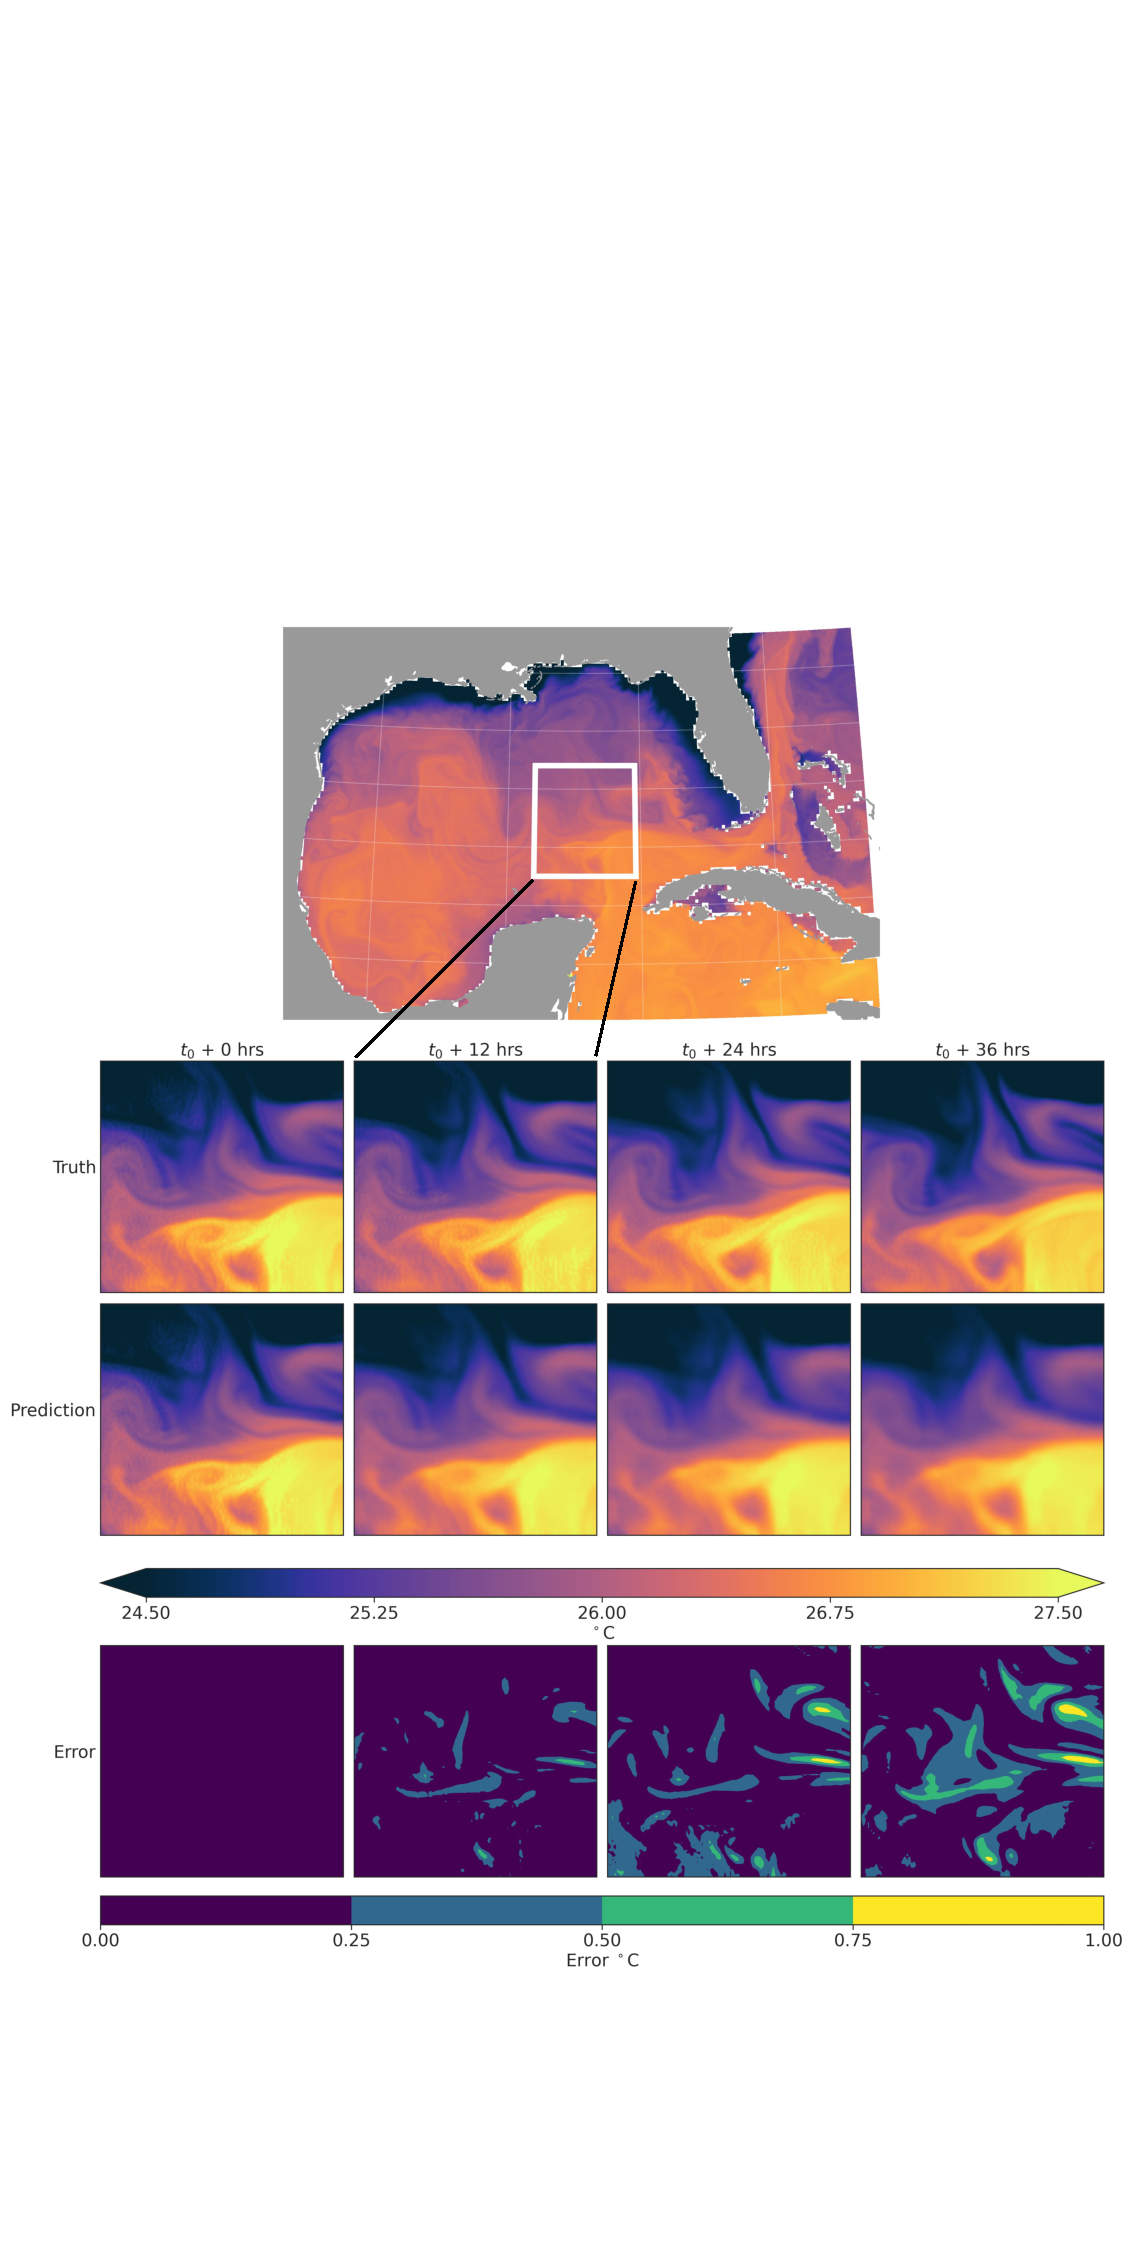
\includegraphics[width=.8\textwidth]{../figures/rc_gom_sst.pdf}
    \caption{A sample prediction of sea surface temperatures in the Gulf of Mexico at 1/25$^\circ$
        horizontal resolution.
        The upper row (Truth) shows the evolution of unseen test data from the
        Navy/HYCOM reanalysis product, and the middle row shows a prediction
        from the Echo State Network architecture described in
        \cref{subsec:rc}.
        The bottom row (Error) shows the absolute value of the difference between the two.
        See \cref{sec:gom} for a description of the dataset.
    }
    \label{fig:gom_sst}
\end{figure}

To make the discussion concrete, we present a sample prediction from our own surrogate model
in \cref{fig:gom_sst}.
The panels show the time evolution of Sea Surface
Temperature (SST) in the Gulf of Mexico at 1/25$^\circ$ horizontal resolution,
using data from a Navy/HYCOM, 3D-Var-based reanalysis product
as ``Truth'' (upper row; see \cref{sec:gom} for data details).
We generate the prediction (middle row) with an RNN architecture
described more fully in \cref{subsec:rc}.
Generally speaking, the RNN captures the largest scales of the SST pattern over
a 36~hour window.
However, as time progresses, the SST pattern becomes overly smooth.
The RNN is
unable to capture the spatial details that are well resolved in the reanalysis
dataset, with the largest errors evolving along sharp SST fronts.
We note that a similar smoothing behavior can be observed in other neural
network based emulators, see for example
\citep<>[Figure 1]{bi_pangu-weather_2022},
\citep<>[Figure 4c \& 4d]{pathak_fourcastnet_2022},
\citep<>[Figure 5]{keisler_forecasting_2022}


There are a number of reasons that could cause this smoothing behavior to manifest in the
predictions.
Our primary goal is to explore at least one reason why this occurs
and explore an optimization based technique to mitigate its effects.
%in order to understand what spatial scales can reliably be resolved.
We note that our example in \cref{fig:gom_sst} and many existing emulators use
reanalysis datasets as training data
\citep<e.g.>[]{lam_graphcast_2022,bi_pangu-weather_2022,pathak_fourcastnet_2022,keisler_forecasting_2022,weyn_sub-seasonal_2021,arcomano_machine_2020}.
There are many excellent reasons to use reanalysis products as training
data; namely they are constrained to observational data.
However, we contend that there are imperfections with reanalysis datasets that
need to be understood in order to be used in data-driven methods.
For instance, reanalyses typically contain jumps in the state vector at the
start of each data assimilation window, and due to the massive size of the data,
they are typically only available at time intervals longer than the timestep
used in the underlying dynamical model.
In our work, we explore the degree to which this simple subsampling step impedes
recurrent and autogregressive neural networks from learning the true underlying
dynamics of the system.
In order to isolate this effect from the potential impacts of a data
assimilation system and multivariate interactions,  we do not rely on the GoM reanalysis data.
Instead, we use a model for Surface Quasi-Geostrophic (SQG) which additionally
gives us direct control over the datasets used for training, validation, and
testing.
The SQG model and dataset generation is described more fully in
\cref{sec:sqg}.

The architectures that we use in this study broadly stem from a braod class of machine
learning techniques termed as reservoir computing (RC),
which was independently discovered as
Echo State Networks \citep<ESNs;>[]{jaeger_echo_2001},
Liquid State Machines \citep{maass_real-time_2002},
and the Decorrelation Backpropagation Rule
\citep{steil_backpropagation-decorrelation_2004}.
%In our work we employ an Echo State Network architecture, and note the work of
%\citet{verstraeten_experimental_2007}, who presented an empirical unification of
%these techniques.
One defining characteristic of RC is that all internal connections are
preset by global or ``macro-scale'' parameters, significantly reducing the
number of parameters that need to be trained.
The relatively simplified structure and training requirements of RC make it an
attractive architecture for large scale prediction because it enables rapid development.
More importantly though, we are motivated to use RC because past studies have
repeatedly shown that it can emulate low dimensional chaotic systems while
remaining competitive with more complex RNNs such as those with Long Short-Term Memory
units (LSTMs)
\citep<e.g.>[]{platt_systematic_2022,vlachas_backpropagation_2020,griffith_forecasting_2019,lu_attractor_2018,pathak_model-free_2018}.
%and emulate atmospheric dynamics with similar skill as a coarse resolution
%primitive equation GCM \citep{arcomano_machine_2020}.
%Here we summarize a few key results.
%\citet{platt_systematic_2022} showed that by systematically optimizing the RC
%hyperparameters, it can emulate the dynamics of a variety of chaotic systems and
%remain on the ``true'' trajectory out to 4-12 times $1/\lambda_1$ on average, where
%$\lambda_1$ is the leading Lyapunov exponent.
%\citet{pathak_using_2017} and \citet{lu_attractor_2018} showed that when a
%well-calibrated RC model
%eventually diverges from the ``truth'' in a chaotic system, the long-term behavior
%resembles a typical trajectory on the attractor, such that RC respects the
%ergodic properties of the underlying system.
%Moreover, \citet{vlachas_backpropagation_2020} showed that RC can outperform more
%complex RNNs like LSTMs in predicting chaotic dynamics, indicating that the
%fixed internal connections could afford some robustness for prediction.
Additionally, \citet{penny_integrating_2022} showed that RC can be
successfully integrated into a number of data assimilation algorithms, either
by generating samples for ensemble based methods like the Ensemble Kalman Filter,
or by generating the tangent linear model necessary for 4D-Var.
Finally, we note that \citet{gauthier_next_2021} proposed a further
simplification to the RC architecture based on insights from
\citet{bollt_explaining_2021} that unifies RC with nonlinear vector
autoregression (NVAR).
For a variety of chaotic systems, this architecture has shown excellent prediction skill
even with low order, polynomial-based feature vectors
\citep{chen_next_2022,barbosa_learning_2022,gauthier_next_2021}, despite requiring a much
smaller hidden state and less training data.
Considering all of these advancements, we explore how well the simple yet
powerful single-layer NVAR and ESN architectures perform in emulating turbulent
geophysical fluid dynamics (see \cref{sec:rnn-architecture} for architecture
details).

%In this work, we probe the following questions more precisely:
%\begin{itemize}
%    \item What spatial scales can be resolved by NN emulators?
%    \item How do fundamental choices in the training data, like temporal
%        subsampling or spatial rescaling, impact the prediction skill?
%    \item How do architectural changes to the network impact prediction skill?
%\end{itemize}
%In the study, we use two forms of RNNs to emulate dynamics relevant to
%geophysical fluids: Reservoir Computing (RC) and a form of Nonlinear Vector
%Auto-Regression (NVAR) that is motivated by the RC paradigm (described
%in \cref{sec:rnn-architecture}).
%Throughout the study, we focus our attention on how well these RNNs can emulate
%turbulent Surface
%Quasi-Geostrophic (SQG) motion (\cref{sec:sqg}).
%We show in \cref{sec:results} that this relatively idealized model exhibits similar
%smoothing behavior as shown in the Gulf of Mexico SST prediction.
%However, using this model allows us to quantify the resolved scales of motion
%more readily, and make changes to the training data, so that we can address the
%questions outlined above.
%While of course we cannot test all NN architectures for emulating these
%dynamics, we discuss the broader implications of our RNN-based results
%for the general setting of NN emulation development for weather and climate
%prediction in \cref{sec:discussion}.
